% Created by tikzDevice version 0.6.1 on 2011-06-27 01:05:23
% !TEX encoding = UTF-8 Unicode
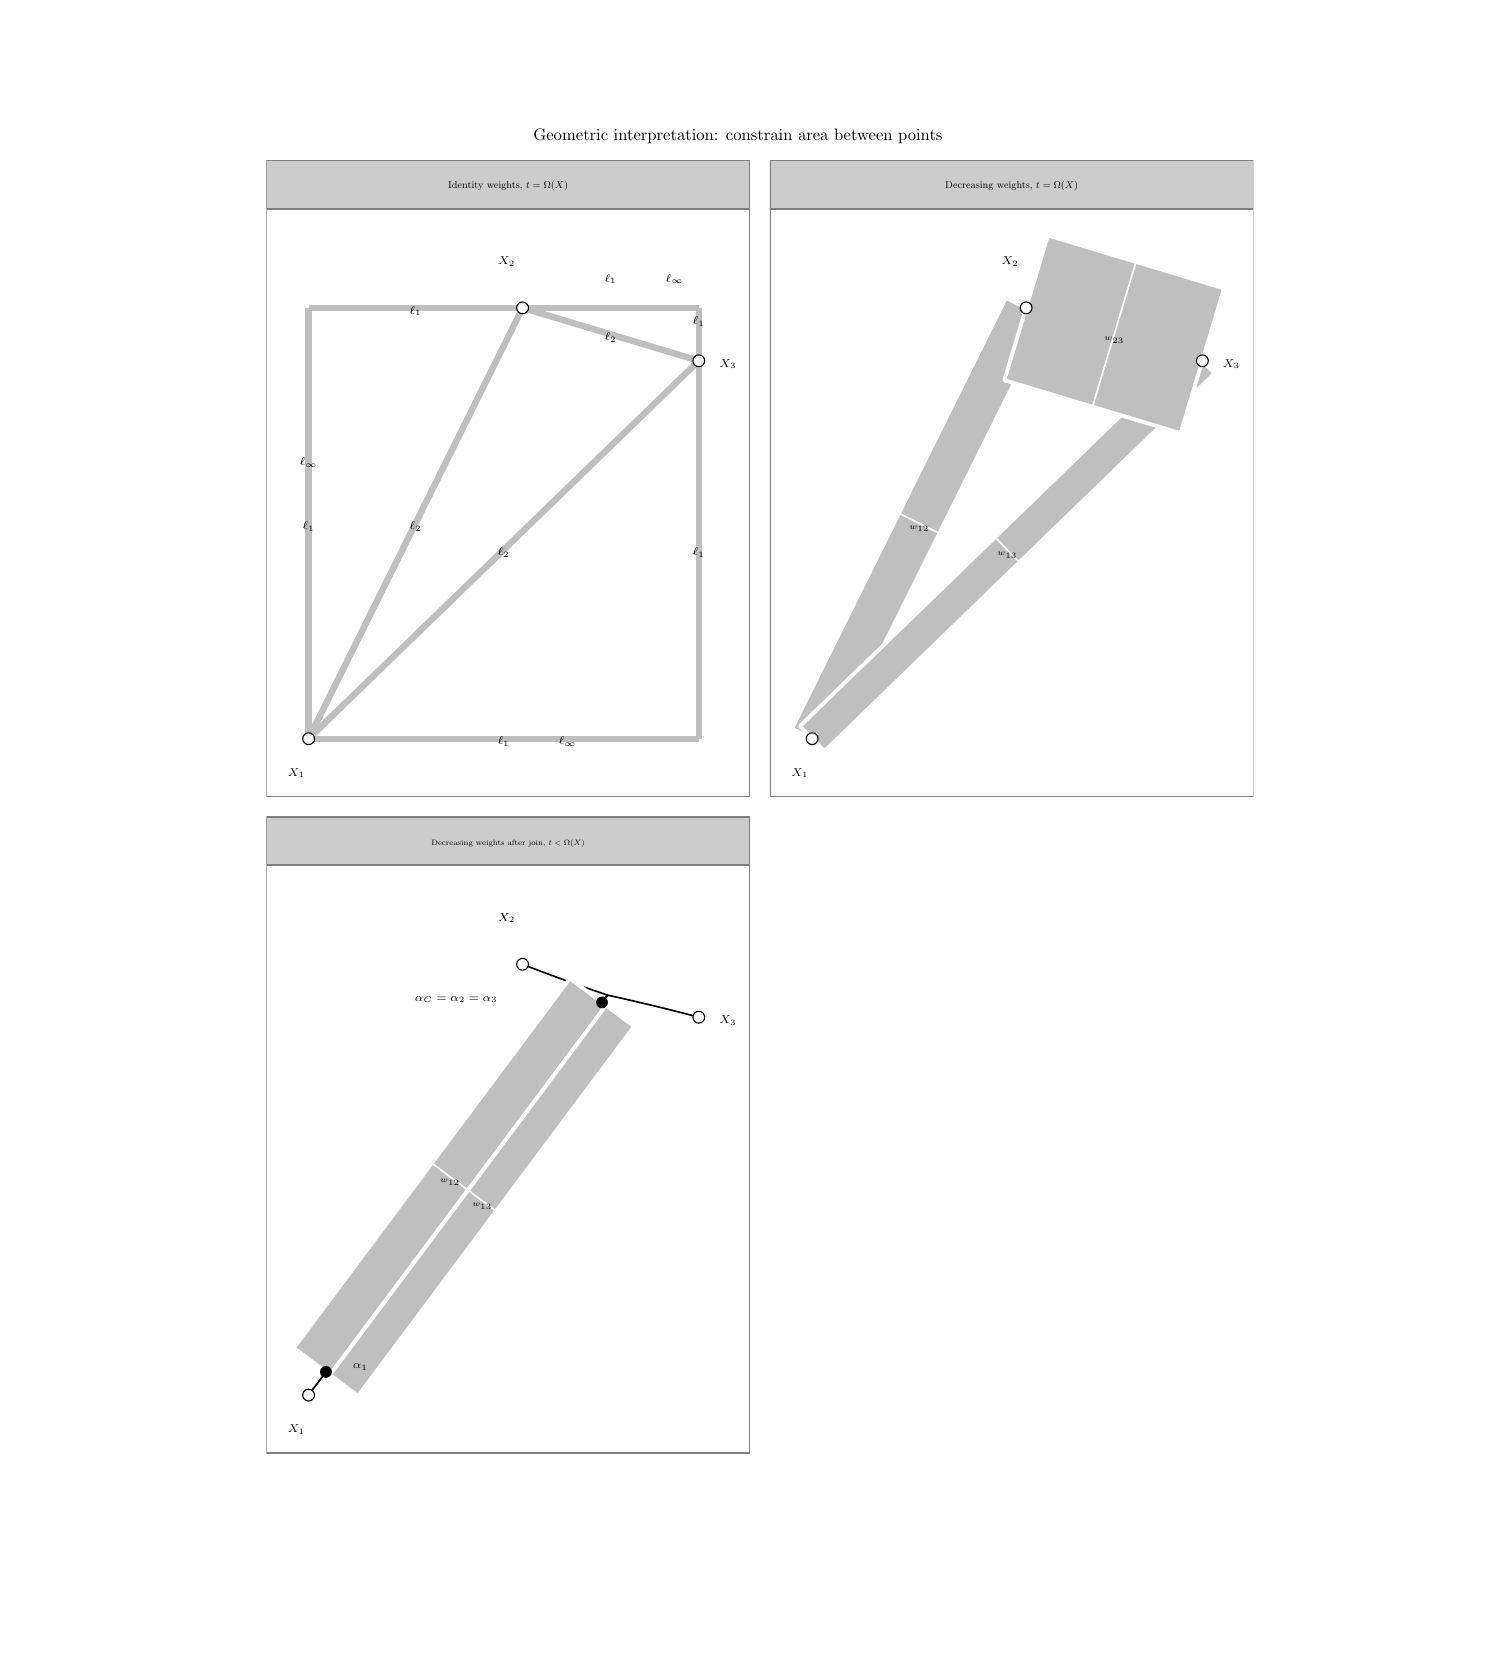
\begin{tikzpicture}[x=1pt,y=1pt]
\definecolor[named]{drawColor}{rgb}{0.00,0.00,0.00}
\definecolor[named]{fillColor}{rgb}{1.00,1.00,1.00}
\fill[color=fillColor,] (0,0) rectangle (523.96,578.16);
\begin{scope}
\path[clip] (  0.00,  0.00) rectangle (523.96,578.16);
\end{scope}
\begin{scope}
\path[clip] (  0.00,  0.00) rectangle (523.96,578.16);
\end{scope}
\begin{scope}
\path[clip] (  0.00,  0.00) rectangle (523.96,578.16);
\end{scope}
\begin{scope}
\path[clip] (  0.00,  0.00) rectangle (523.96,578.16);
\end{scope}
\begin{scope}
\path[clip] (  0.00,  0.00) rectangle (523.96,578.16);
\end{scope}
\begin{scope}
\path[clip] (  0.00,  0.00) rectangle (523.96,578.16);
\end{scope}
\begin{scope}
\path[clip] (  0.00,  0.00) rectangle (523.96,578.16);
\end{scope}
\begin{scope}
\path[clip] (  0.00,  0.00) rectangle (523.96,578.16);
\end{scope}
\begin{scope}
\path[clip] (  0.00,  0.00) rectangle (523.96,578.16);
\end{scope}
\begin{scope}
\path[clip] (  0.00,  0.00) rectangle (523.96,578.16);
\end{scope}
\begin{scope}
\path[clip] (  0.00,  0.00) rectangle (523.96,578.16);
\end{scope}
\begin{scope}
\path[clip] (  0.00,  0.00) rectangle (523.96,578.16);
\end{scope}
\begin{scope}
\path[clip] (  0.00,  0.00) rectangle (523.96,578.16);

\draw[fill opacity=0.00,draw opacity=0.00,] (  0.00,  0.00) rectangle (523.96,578.16);
\end{scope}
\begin{scope}
\path[clip] (  0.00,  0.00) rectangle (523.96,578.16);
\definecolor[named]{drawColor}{rgb}{0.00,0.00,0.00}

\node[color=drawColor,anchor=base,inner sep=0pt, outer sep=0pt, scale=  0.60] at (256.65,537.46) {Geometric interpretation: constrain area between points%
};
\end{scope}
\begin{scope}
\path[clip] (  0.00,  0.00) rectangle (523.96,578.16);
\end{scope}
\begin{scope}
\path[clip] (  0.00,  0.00) rectangle (523.96,578.16);
\end{scope}
\begin{scope}
\path[clip] (  0.00,  0.00) rectangle (523.96,578.16);
\end{scope}
\begin{scope}
\path[clip] ( 63.13,512.74) rectangle ( 86.26,530.24);
\end{scope}
\begin{scope}
\path[clip] (  0.00,  0.00) rectangle (523.96,578.16);
\end{scope}
\begin{scope}
\path[clip] (  0.00,  0.00) rectangle (523.96,578.16);
\end{scope}
\begin{scope}
\path[clip] (  0.00,  0.00) rectangle (523.96,578.16);
\end{scope}
\begin{scope}
\path[clip] ( 63.13,300.26) rectangle ( 86.26,300.26);
\end{scope}
\begin{scope}
\path[clip] (  0.00,  0.00) rectangle (523.96,578.16);
\end{scope}
\begin{scope}
\path[clip] ( 63.13,293.04) rectangle ( 86.26,300.26);
\end{scope}
\begin{scope}
\path[clip] (  0.00,  0.00) rectangle (523.96,578.16);
\end{scope}
\begin{scope}
\path[clip] ( 63.13,275.54) rectangle ( 86.26,293.04);
\end{scope}
\begin{scope}
\path[clip] (  0.00,  0.00) rectangle (523.96,578.16);
\end{scope}
\begin{scope}
\path[clip] (  0.00,  0.00) rectangle (523.96,578.16);
\end{scope}
\begin{scope}
\path[clip] (  0.00,  0.00) rectangle (523.96,578.16);
\end{scope}
\begin{scope}
\path[clip] ( 63.13, 39.94) rectangle ( 86.26, 63.06);
\end{scope}
\begin{scope}
\path[clip] (  0.00,  0.00) rectangle (523.96,578.16);
\end{scope}
\begin{scope}
\path[clip] ( 63.13, 32.71) rectangle ( 86.26, 39.94);
\end{scope}
\begin{scope}
\path[clip] (  0.00,  0.00) rectangle (523.96,578.16);
\end{scope}
\begin{scope}
\path[clip] ( 86.26,512.74) rectangle (260.99,530.24);
\end{scope}
\begin{scope}
\path[clip] (  0.00,  0.00) rectangle (523.96,578.16);
\end{scope}
\begin{scope}
\path[clip] ( 86.26,300.26) rectangle (260.99,512.74);
\end{scope}
\begin{scope}
\path[clip] (  0.00,  0.00) rectangle (523.96,578.16);
\end{scope}
\begin{scope}
\path[clip] ( 86.26,300.26) rectangle (260.99,300.26);
\end{scope}
\begin{scope}
\path[clip] (  0.00,  0.00) rectangle (523.96,578.16);
\end{scope}
\begin{scope}
\path[clip] ( 86.26,293.04) rectangle (260.99,300.26);
\end{scope}
\begin{scope}
\path[clip] (  0.00,  0.00) rectangle (523.96,578.16);
\end{scope}
\begin{scope}
\path[clip] ( 86.26,275.54) rectangle (260.99,293.04);
\end{scope}
\begin{scope}
\path[clip] (  0.00,  0.00) rectangle (523.96,578.16);
\end{scope}
\begin{scope}
\path[clip] ( 86.26, 63.06) rectangle (260.99,275.54);
\end{scope}
\begin{scope}
\path[clip] (  0.00,  0.00) rectangle (523.96,578.16);
\end{scope}
\begin{scope}
\path[clip] (  0.00,  0.00) rectangle (523.96,578.16);
\end{scope}
\begin{scope}
\path[clip] (  0.00,  0.00) rectangle (523.96,578.16);
\end{scope}
\begin{scope}
\path[clip] ( 86.26, 32.71) rectangle (260.99, 39.94);
\end{scope}
\begin{scope}
\path[clip] (  0.00,  0.00) rectangle (523.96,578.16);
\end{scope}
\begin{scope}
\path[clip] (260.99,512.74) rectangle (268.22,530.24);
\end{scope}
\begin{scope}
\path[clip] (  0.00,  0.00) rectangle (523.96,578.16);
\end{scope}
\begin{scope}
\path[clip] (260.99,300.26) rectangle (268.22,512.74);
\end{scope}
\begin{scope}
\path[clip] (  0.00,  0.00) rectangle (523.96,578.16);
\end{scope}
\begin{scope}
\path[clip] (260.99,300.26) rectangle (268.22,300.26);
\end{scope}
\begin{scope}
\path[clip] (  0.00,  0.00) rectangle (523.96,578.16);
\end{scope}
\begin{scope}
\path[clip] (260.99,293.04) rectangle (268.22,300.26);
\end{scope}
\begin{scope}
\path[clip] (  0.00,  0.00) rectangle (523.96,578.16);
\end{scope}
\begin{scope}
\path[clip] (260.99,275.54) rectangle (268.22,293.04);
\end{scope}
\begin{scope}
\path[clip] (  0.00,  0.00) rectangle (523.96,578.16);
\end{scope}
\begin{scope}
\path[clip] (260.99, 63.06) rectangle (268.22,275.54);
\end{scope}
\begin{scope}
\path[clip] (  0.00,  0.00) rectangle (523.96,578.16);
\end{scope}
\begin{scope}
\path[clip] (260.99, 39.94) rectangle (268.22, 63.06);
\end{scope}
\begin{scope}
\path[clip] (  0.00,  0.00) rectangle (523.96,578.16);
\end{scope}
\begin{scope}
\path[clip] (260.99, 32.71) rectangle (268.22, 39.94);
\end{scope}
\begin{scope}
\path[clip] (  0.00,  0.00) rectangle (523.96,578.16);
\end{scope}
\begin{scope}
\path[clip] (268.22,512.74) rectangle (268.22,530.24);
\end{scope}
\begin{scope}
\path[clip] (  0.00,  0.00) rectangle (523.96,578.16);
\end{scope}
\begin{scope}
\path[clip] (268.22,300.26) rectangle (268.22,512.74);
\end{scope}
\begin{scope}
\path[clip] (  0.00,  0.00) rectangle (523.96,578.16);
\end{scope}
\begin{scope}
\path[clip] (268.22,300.26) rectangle (268.22,300.26);
\end{scope}
\begin{scope}
\path[clip] (  0.00,  0.00) rectangle (523.96,578.16);
\end{scope}
\begin{scope}
\path[clip] (268.22,293.04) rectangle (268.22,300.26);
\end{scope}
\begin{scope}
\path[clip] (  0.00,  0.00) rectangle (523.96,578.16);
\end{scope}
\begin{scope}
\path[clip] (268.22,275.54) rectangle (268.22,293.04);
\end{scope}
\begin{scope}
\path[clip] (  0.00,  0.00) rectangle (523.96,578.16);
\end{scope}
\begin{scope}
\path[clip] (268.22, 63.06) rectangle (268.22,275.54);
\end{scope}
\begin{scope}
\path[clip] (  0.00,  0.00) rectangle (523.96,578.16);
\end{scope}
\begin{scope}
\path[clip] (268.22, 39.94) rectangle (268.22, 63.06);
\end{scope}
\begin{scope}
\path[clip] (  0.00,  0.00) rectangle (523.96,578.16);
\end{scope}
\begin{scope}
\path[clip] (268.22, 32.71) rectangle (268.22, 39.94);
\end{scope}
\begin{scope}
\path[clip] (  0.00,  0.00) rectangle (523.96,578.16);
\end{scope}
\begin{scope}
\path[clip] (268.22,512.74) rectangle (442.94,530.24);
\end{scope}
\begin{scope}
\path[clip] (  0.00,  0.00) rectangle (523.96,578.16);
\end{scope}
\begin{scope}
\path[clip] (268.22,300.26) rectangle (442.94,512.74);
\end{scope}
\begin{scope}
\path[clip] (  0.00,  0.00) rectangle (523.96,578.16);
\end{scope}
\begin{scope}
\path[clip] (268.22,300.26) rectangle (442.94,300.26);
\end{scope}
\begin{scope}
\path[clip] (  0.00,  0.00) rectangle (523.96,578.16);
\end{scope}
\begin{scope}
\path[clip] (268.22,293.04) rectangle (442.94,300.26);
\end{scope}
\begin{scope}
\path[clip] (  0.00,  0.00) rectangle (523.96,578.16);
\end{scope}
\begin{scope}
\path[clip] (268.22,275.54) rectangle (442.94,293.04);
\end{scope}
\begin{scope}
\path[clip] (  0.00,  0.00) rectangle (523.96,578.16);
\end{scope}
\begin{scope}
\path[clip] (268.22, 63.06) rectangle (442.94,275.54);
\end{scope}
\begin{scope}
\path[clip] (  0.00,  0.00) rectangle (523.96,578.16);
\end{scope}
\begin{scope}
\path[clip] (  0.00,  0.00) rectangle (523.96,578.16);
\end{scope}
\begin{scope}
\path[clip] (  0.00,  0.00) rectangle (523.96,578.16);
\end{scope}
\begin{scope}
\path[clip] (268.22, 32.71) rectangle (442.94, 39.94);
\end{scope}
\begin{scope}
\path[clip] (  0.00,  0.00) rectangle (523.96,578.16);
\end{scope}
\begin{scope}
\path[clip] (442.94,512.74) rectangle (450.17,530.24);
\end{scope}
\begin{scope}
\path[clip] (  0.00,  0.00) rectangle (523.96,578.16);
\end{scope}
\begin{scope}
\path[clip] (442.94,300.26) rectangle (450.17,512.74);
\end{scope}
\begin{scope}
\path[clip] (  0.00,  0.00) rectangle (523.96,578.16);
\end{scope}
\begin{scope}
\path[clip] (442.94,300.26) rectangle (450.17,300.26);
\end{scope}
\begin{scope}
\path[clip] (  0.00,  0.00) rectangle (523.96,578.16);
\end{scope}
\begin{scope}
\path[clip] (442.94,293.04) rectangle (450.17,300.26);
\end{scope}
\begin{scope}
\path[clip] (  0.00,  0.00) rectangle (523.96,578.16);
\end{scope}
\begin{scope}
\path[clip] (442.94,275.54) rectangle (450.17,293.04);
\end{scope}
\begin{scope}
\path[clip] (  0.00,  0.00) rectangle (523.96,578.16);
\end{scope}
\begin{scope}
\path[clip] (442.94, 63.06) rectangle (450.17,275.54);
\end{scope}
\begin{scope}
\path[clip] (  0.00,  0.00) rectangle (523.96,578.16);
\end{scope}
\begin{scope}
\path[clip] (442.94, 39.94) rectangle (450.17, 63.06);
\end{scope}
\begin{scope}
\path[clip] (  0.00,  0.00) rectangle (523.96,578.16);
\end{scope}
\begin{scope}
\path[clip] (442.94, 32.71) rectangle (450.17, 39.94);
\end{scope}
\begin{scope}
\path[clip] (  0.00,  0.00) rectangle (523.96,578.16);
\end{scope}
\begin{scope}
\path[clip] ( 63.13,512.74) rectangle ( 86.26,530.24);
\end{scope}
\begin{scope}
\path[clip] (  0.00,  0.00) rectangle (523.96,578.16);
\end{scope}
\begin{scope}
\path[clip] (  0.00,  0.00) rectangle (523.96,578.16);
\end{scope}
\begin{scope}
\path[clip] (  0.00,  0.00) rectangle (523.96,578.16);
\end{scope}
\begin{scope}
\path[clip] (  0.00,  0.00) rectangle (523.96,578.16);
\end{scope}
\begin{scope}
\path[clip] (  0.00,  0.00) rectangle (523.96,578.16);
\end{scope}
\begin{scope}
\path[clip] (  0.00,  0.00) rectangle (523.96,578.16);
\end{scope}
\begin{scope}
\path[clip] ( 63.13,300.26) rectangle ( 86.26,300.26);
\end{scope}
\begin{scope}
\path[clip] (  0.00,  0.00) rectangle (523.96,578.16);
\end{scope}
\begin{scope}
\path[clip] ( 63.13,293.04) rectangle ( 86.26,300.26);
\end{scope}
\begin{scope}
\path[clip] (  0.00,  0.00) rectangle (523.96,578.16);
\end{scope}
\begin{scope}
\path[clip] ( 63.13,275.54) rectangle ( 86.26,293.04);
\end{scope}
\begin{scope}
\path[clip] (  0.00,  0.00) rectangle (523.96,578.16);
\end{scope}
\begin{scope}
\path[clip] (  0.00,  0.00) rectangle (523.96,578.16);
\end{scope}
\begin{scope}
\path[clip] (  0.00,  0.00) rectangle (523.96,578.16);
\end{scope}
\begin{scope}
\path[clip] (  0.00,  0.00) rectangle (523.96,578.16);
\end{scope}
\begin{scope}
\path[clip] (  0.00,  0.00) rectangle (523.96,578.16);
\end{scope}
\begin{scope}
\path[clip] (  0.00,  0.00) rectangle (523.96,578.16);
\end{scope}
\begin{scope}
\path[clip] ( 63.13, 39.94) rectangle ( 86.26, 63.06);
\end{scope}
\begin{scope}
\path[clip] (  0.00,  0.00) rectangle (523.96,578.16);
\end{scope}
\begin{scope}
\path[clip] ( 63.13, 32.71) rectangle ( 86.26, 39.94);
\end{scope}
\begin{scope}
\path[clip] (  0.00,  0.00) rectangle (523.96,578.16);
\end{scope}
\begin{scope}
\path[clip] ( 86.26,512.74) rectangle (260.99,530.24);
\definecolor[named]{drawColor}{rgb}{0.50,0.50,0.50}
\definecolor[named]{fillColor}{rgb}{0.80,0.80,0.80}

\draw[color=drawColor,line width= 0.6pt,line cap=round,line join=round,fill=fillColor,] ( 86.26,512.74) rectangle (260.99,530.24);
\definecolor[named]{drawColor}{rgb}{0.00,0.00,0.00}

\node[color=drawColor,anchor=base,inner sep=0pt, outer sep=0pt, scale=  0.40] at (173.62,519.97) {\small Identity weights, $t=\Omega(X)$%
};
\end{scope}
\begin{scope}
\path[clip] (  0.00,  0.00) rectangle (523.96,578.16);
\end{scope}
\begin{scope}
\path[clip] ( 86.26,300.26) rectangle (260.99,512.74);
\definecolor[named]{fillColor}{rgb}{1.00,1.00,1.00}

\draw[fill=fillColor,draw opacity=0.00,] ( 86.26,300.26) rectangle (260.99,512.74);
\definecolor[named]{drawColor}{rgb}{0.75,0.75,0.75}

\draw[color=drawColor,line width= 2.3pt,line join=round,fill opacity=0.00,] (101.51,321.23) -- (101.51,476.91);

\draw[color=drawColor,line width= 2.3pt,line join=round,fill opacity=0.00,] (178.83,476.91) -- (101.51,476.91);

\draw[color=drawColor,line width= 2.3pt,line join=round,fill opacity=0.00,] (242.51,457.78) -- (242.51,476.91);

\draw[color=drawColor,line width= 2.3pt,line join=round,fill opacity=0.00,] (101.51,321.23) -- (242.51,321.23);

\draw[color=drawColor,line width= 2.3pt,line join=round,fill opacity=0.00,] (178.83,476.91) -- (242.51,476.91);

\draw[color=drawColor,line width= 2.3pt,line join=round,fill opacity=0.00,] (242.51,457.78) -- (242.51,321.23);

\draw[color=drawColor,line width= 2.3pt,line join=round,fill opacity=0.00,] (101.51,321.23) -- (178.83,476.91);

\draw[color=drawColor,line width= 2.3pt,line join=round,fill opacity=0.00,] (101.51,321.23) -- (242.51,457.78);

\draw[color=drawColor,line width= 2.3pt,line join=round,fill opacity=0.00,] (178.83,476.91) -- (242.51,457.78);
\definecolor[named]{drawColor}{rgb}{0.00,0.00,0.00}

\node[color=drawColor,anchor=base,inner sep=0pt, outer sep=0pt, scale=  0.59] at (140.17,396.82) {\scriptsize$\ell_2$%
};

\node[color=drawColor,anchor=base,inner sep=0pt, outer sep=0pt, scale=  0.59] at (172.01,387.26) {\scriptsize$\ell_2$%
};

\node[color=drawColor,anchor=base,inner sep=0pt, outer sep=0pt, scale=  0.59] at (210.67,465.10) {\scriptsize$\ell_2$%
};

\node[color=drawColor,anchor=base,inner sep=0pt, outer sep=0pt, scale=  0.59] at (101.51,396.82) {\scriptsize$\ell_1$%
};

\node[color=drawColor,anchor=base,inner sep=0pt, outer sep=0pt, scale=  0.59] at (140.17,474.67) {\scriptsize$\ell_1$%
};

\node[color=drawColor,anchor=base,inner sep=0pt, outer sep=0pt, scale=  0.59] at (242.51,470.88) {\scriptsize$\ell_1$%
};

\node[color=drawColor,anchor=base,inner sep=0pt, outer sep=0pt, scale=  0.59] at (172.01,318.98) {\scriptsize$\ell_1$%
};

\node[color=drawColor,anchor=base,inner sep=0pt, outer sep=0pt, scale=  0.59] at (210.67,486.22) {\scriptsize$\ell_1$%
};

\node[color=drawColor,anchor=base,inner sep=0pt, outer sep=0pt, scale=  0.59] at (242.51,387.26) {\scriptsize$\ell_1$%
};

\node[color=drawColor,anchor=base,inner sep=0pt, outer sep=0pt, scale=  0.59] at (101.51,419.93) {\scriptsize$\ell_\infty$%
};

\node[color=drawColor,anchor=base,inner sep=0pt, outer sep=0pt, scale=  0.59] at (195.11,318.98) {\scriptsize$\ell_\infty$%
};

\node[color=drawColor,anchor=base,inner sep=0pt, outer sep=0pt, scale=  0.59] at (233.77,486.22) {\scriptsize$\ell_\infty$%
};

\node[color=drawColor,anchor=base,inner sep=0pt, outer sep=0pt, scale=  0.59] at ( 97.12,307.68) {\scriptsize$X_1$%
};

\node[color=drawColor,anchor=base,inner sep=0pt, outer sep=0pt, scale=  0.59] at (173.06,492.48) {\scriptsize$X_2$%
};

\node[color=drawColor,anchor=base,inner sep=0pt, outer sep=0pt, scale=  0.59] at (253.05,455.53) {\scriptsize$X_3$%
};

\draw[color=drawColor,line cap=round,line join=round,fill=fillColor,] (101.51,321.23) circle (  2.13);

\draw[color=drawColor,line cap=round,line join=round,fill=fillColor,] (178.83,476.91) circle (  2.13);

\draw[color=drawColor,line cap=round,line join=round,fill=fillColor,] (242.51,457.78) circle (  2.13);
\definecolor[named]{drawColor}{rgb}{0.50,0.50,0.50}

\draw[color=drawColor,line width= 0.6pt,line cap=round,line join=round,fill opacity=0.00,] ( 86.26,300.26) rectangle (260.99,512.74);
\end{scope}
\begin{scope}
\path[clip] (  0.00,  0.00) rectangle (523.96,578.16);
\end{scope}
\begin{scope}
\path[clip] ( 86.26,300.26) rectangle (260.99,300.26);
\end{scope}
\begin{scope}
\path[clip] (  0.00,  0.00) rectangle (523.96,578.16);
\end{scope}
\begin{scope}
\path[clip] ( 86.26,293.04) rectangle (260.99,300.26);
\end{scope}
\begin{scope}
\path[clip] (  0.00,  0.00) rectangle (523.96,578.16);
\end{scope}
\begin{scope}
\path[clip] ( 86.26,275.54) rectangle (260.99,293.04);
\definecolor[named]{drawColor}{rgb}{0.50,0.50,0.50}
\definecolor[named]{fillColor}{rgb}{0.80,0.80,0.80}

\draw[color=drawColor,line width= 0.6pt,line cap=round,line join=round,fill=fillColor,] ( 86.26,275.54) rectangle (260.99,293.04);
\definecolor[named]{drawColor}{rgb}{0.00,0.00,0.00}

\node[color=drawColor,anchor=base,inner sep=0pt, outer sep=0pt, scale=  0.40] at (173.62,282.77) {\scriptsize Decreasing weights after join, $t<\Omega(X)$%
};
\end{scope}
\begin{scope}
\path[clip] (  0.00,  0.00) rectangle (523.96,578.16);
\end{scope}
\begin{scope}
\path[clip] ( 86.26, 63.06) rectangle (260.99,275.54);
\definecolor[named]{fillColor}{rgb}{1.00,1.00,1.00}

\draw[fill=fillColor,draw opacity=0.00,] ( 86.26, 63.06) rectangle (260.99,275.54);
\definecolor[named]{drawColor}{rgb}{0.00,0.00,0.00}

\draw[color=drawColor,line width= 0.6pt,line join=round,fill opacity=0.00,] (101.51, 84.03) --
	(101.56, 84.10) --
	(101.56, 84.10) --
	(101.57, 84.11) --
	(101.57, 84.11) --
	(101.57, 84.11) --
	(101.57, 84.12) --
	(101.58, 84.12) --
	(101.58, 84.13) --
	(101.58, 84.13) --
	(101.59, 84.14) --
	(101.59, 84.14) --
	(101.59, 84.15) --
	(101.60, 84.16) --
	(101.60, 84.16) --
	(101.61, 84.17) --
	(101.61, 84.18) --
	(101.62, 84.18) --
	(101.62, 84.19) --
	(101.63, 84.20) --
	(101.63, 84.21) --
	(101.64, 84.22) --
	(101.64, 84.23) --
	(101.65, 84.24) --
	(101.66, 84.25) --
	(101.67, 84.26) --
	(101.67, 84.27) --
	(101.68, 84.29) --
	(101.69, 84.30) --
	(101.70, 84.31) --
	(101.71, 84.33) --
	(101.72, 84.34) --
	(101.73, 84.36) --
	(101.74, 84.37) --
	(101.75, 84.39) --
	(101.76, 84.41) --
	(101.78, 84.43) --
	(101.79, 84.45) --
	(101.80, 84.47) --
	(101.82, 84.49) --
	(101.83, 84.51) --
	(101.85, 84.54) --
	(101.87, 84.56) --
	(101.88, 84.59) --
	(101.90, 84.62) --
	(101.92, 84.65) --
	(101.94, 84.68) --
	(101.97, 84.71) --
	(101.99, 84.75) --
	(102.01, 84.78) --
	(102.04, 84.82) --
	(102.07, 84.86) --
	(102.10, 84.90) --
	(102.13, 84.94) --
	(102.16, 84.99) --
	(102.19, 85.04) --
	(102.23, 85.09) --
	(102.26, 85.14) --
	(102.30, 85.19) --
	(102.35, 85.25) --
	(102.39, 85.31) --
	(102.43, 85.37) --
	(102.48, 85.44) --
	(102.53, 85.51) --
	(102.59, 85.58) --
	(102.65, 85.66) --
	(102.71, 85.74) --
	(102.77, 85.82) --
	(102.84, 85.91) --
	(102.91, 86.00) --
	(102.98, 86.10) --
	(103.06, 86.20) --
	(103.15, 86.30) --
	(103.23, 86.41) --
	(103.33, 86.53) --
	(103.42, 86.65) --
	(103.53, 86.78) --
	(103.64, 86.91) --
	(103.75, 87.05) --
	(103.88, 87.19) --
	(104.00, 87.35) --
	(104.12, 87.51) --
	(104.25, 87.69) --
	(104.39, 87.87) --
	(104.53, 88.06) --
	(104.68, 88.26) --
	(104.84, 88.48) --
	(105.01, 88.70) --
	(105.18, 88.93) --
	(105.36, 89.18) --
	(105.56, 89.44) --
	(105.76, 89.71) --
	(105.97, 89.99) --
	(106.19, 90.29) --
	(106.43, 90.60) --
	(106.67, 90.93) --
	(106.93, 91.28) --
	(107.20, 91.64) --
	(107.49, 92.02) --
	(107.78, 92.42);

\draw[color=drawColor,line width= 0.6pt,line join=round,fill opacity=0.00,] (178.83,239.71) --
	(179.52,239.44) --
	(179.56,239.43) --
	(179.60,239.42) --
	(179.63,239.40) --
	(179.67,239.39) --
	(179.72,239.37) --
	(179.76,239.35) --
	(179.81,239.33) --
	(179.85,239.32) --
	(179.91,239.30) --
	(179.96,239.27) --
	(180.02,239.25) --
	(180.07,239.23) --
	(180.14,239.21) --
	(180.20,239.18) --
	(180.27,239.15) --
	(180.34,239.13) --
	(180.42,239.10) --
	(180.50,239.07) --
	(180.58,239.03) --
	(180.67,239.00) --
	(180.76,238.96) --
	(180.86,238.93) --
	(180.96,238.89) --
	(181.06,238.85) --
	(181.17,238.80) --
	(181.29,238.76) --
	(181.41,238.71) --
	(181.54,238.66) --
	(181.68,238.61) --
	(181.82,238.55) --
	(181.97,238.50) --
	(182.13,238.44) --
	(182.29,238.37) --
	(182.46,238.31) --
	(182.65,238.24) --
	(182.84,238.16) --
	(183.04,238.09) --
	(183.25,238.01) --
	(183.47,237.92) --
	(183.70,237.83) --
	(183.94,237.74) --
	(184.20,237.64) --
	(184.46,237.54) --
	(184.75,237.44) --
	(185.04,237.32) --
	(185.35,237.21) --
	(185.68,237.08) --
	(186.02,236.95) --
	(186.38,236.82) --
	(186.75,236.68) --
	(187.15,236.53) --
	(187.56,236.37) --
	(188.00,236.21) --
	(188.46,236.04) --
	(188.94,235.86) --
	(189.44,235.67) --
	(189.97,235.48) --
	(190.52,235.27) --
	(191.11,235.06) --
	(191.72,234.83) --
	(192.36,234.60) --
	(193.04,234.35) --
	(193.74,234.09) --
	(194.49,233.83) --
	(195.27,233.54) --
	(196.09,233.25) --
	(196.94,232.95) --
	(197.85,232.63) --
	(198.79,232.28) --
	(199.79,231.94) --
	(200.83,231.57) --
	(201.92,231.18) --
	(203.07,230.78) --
	(204.27,230.36) --
	(205.54,229.93) --
	(206.86,229.47) --
	(208.25,229.00) --
	(209.49,228.57) --
	(209.43,228.49) --
	(209.37,228.40) --
	(209.30,228.32) --
	(209.24,228.22) --
	(209.16,228.13) --
	(209.09,228.03) --
	(209.01,227.92) --
	(208.93,227.81) --
	(208.84,227.69) --
	(208.75,227.57) --
	(208.65,227.44) --
	(208.55,227.31) --
	(208.44,227.16) --
	(208.33,227.02) --
	(208.22,226.86) --
	(208.09,226.69) --
	(207.96,226.52) --
	(207.83,226.34) --
	(207.69,226.15) --
	(207.54,225.95);

\draw[color=drawColor,line width= 0.6pt,line join=round,fill opacity=0.00,] (242.51,220.58) --
	(241.77,220.78) --
	(241.74,220.79) --
	(241.70,220.80) --
	(241.66,220.81) --
	(241.61,220.82) --
	(241.57,220.83) --
	(241.52,220.84) --
	(241.47,220.86) --
	(241.42,220.87) --
	(241.37,220.88) --
	(241.31,220.90) --
	(241.25,220.92) --
	(241.19,220.93) --
	(241.12,220.95) --
	(241.05,220.97) --
	(240.98,220.99) --
	(240.90,221.01) --
	(240.82,221.03) --
	(240.73,221.05) --
	(240.65,221.08) --
	(240.55,221.10) --
	(240.45,221.13) --
	(240.35,221.15) --
	(240.24,221.18) --
	(240.13,221.21) --
	(240.01,221.24) --
	(239.89,221.28) --
	(239.75,221.31) --
	(239.62,221.35) --
	(239.47,221.38) --
	(239.32,221.42) --
	(239.16,221.47) --
	(238.99,221.51) --
	(238.82,221.56) --
	(238.63,221.60) --
	(238.44,221.65) --
	(238.23,221.71) --
	(238.02,221.76) --
	(237.79,221.82) --
	(237.56,221.88) --
	(237.31,221.95) --
	(237.05,222.01) --
	(236.78,222.08) --
	(236.49,222.16) --
	(236.19,222.24) --
	(235.87,222.32) --
	(235.54,222.40) --
	(235.19,222.49) --
	(234.83,222.58) --
	(234.44,222.68) --
	(234.04,222.78) --
	(233.61,222.89) --
	(233.17,223.00) --
	(232.70,223.12) --
	(232.21,223.24) --
	(231.69,223.37) --
	(231.15,223.51) --
	(230.58,223.65) --
	(229.99,223.80) --
	(229.36,223.95) --
	(228.70,224.11) --
	(228.01,224.28) --
	(227.29,224.46) --
	(226.52,224.64) --
	(225.72,224.83) --
	(224.88,225.04) --
	(224.00,225.24) --
	(223.08,225.46) --
	(222.10,225.69) --
	(221.08,225.94) --
	(220.01,226.18) --
	(218.89,226.45) --
	(217.70,226.72) --
	(216.46,227.01) --
	(215.16,227.31) --
	(213.79,227.61) --
	(212.36,227.94) --
	(210.86,228.27) --
	(209.49,228.57) --
	(209.43,228.49) --
	(209.37,228.40) --
	(209.30,228.32) --
	(209.24,228.22) --
	(209.16,228.13) --
	(209.09,228.03) --
	(209.01,227.92) --
	(208.93,227.81) --
	(208.84,227.69) --
	(208.75,227.57) --
	(208.65,227.44) --
	(208.55,227.31) --
	(208.44,227.16) --
	(208.33,227.02) --
	(208.22,226.86) --
	(208.09,226.69) --
	(207.96,226.52) --
	(207.83,226.34) --
	(207.69,226.15) --
	(207.54,225.95);
\definecolor[named]{drawColor}{rgb}{1.00,1.00,1.00}
\definecolor[named]{fillColor}{rgb}{0.75,0.75,0.75}

\draw[color=drawColor,line width= 1.4pt,line cap=round,line join=round,fill=fillColor,] ( 96.16,101.10) --
	(109.24, 91.33) --
	(209.00,224.86) --
	(195.92,234.63) --
	cycle;

\draw[color=drawColor,line width= 1.4pt,line cap=round,line join=round,fill=fillColor,] (109.24, 91.33) --
	(119.40, 83.74) --
	(219.16,217.27) --
	(209.00,224.86) --
	cycle;

\draw[color=drawColor,line width= 0.6pt,line join=round,fill opacity=0.00,] (146.04,167.86) -- (159.12,158.09);

\draw[color=drawColor,line width= 0.6pt,line join=round,fill opacity=0.00,] (159.12,158.09) -- (169.28,150.50);
\definecolor[named]{drawColor}{rgb}{0.00,0.00,0.00}

\node[color=drawColor,anchor=base,inner sep=0pt, outer sep=0pt, scale=  0.59] at (152.58,160.73) {\tiny$w_{12}$%
};

\node[color=drawColor,anchor=base,inner sep=0pt, outer sep=0pt, scale=  0.59] at (164.20,152.05) {\tiny$w_{13}$%
};
\definecolor[named]{fillColor}{rgb}{0.00,0.00,0.00}

\draw[fill=fillColor,draw opacity=0.00,] (107.78, 92.42) circle (  2.13);

\draw[fill=fillColor,draw opacity=0.00,] (207.54,225.95) circle (  2.13);

\node[color=drawColor,anchor=base,inner sep=0pt, outer sep=0pt, scale=  0.59] at ( 97.12, 70.48) {\scriptsize$X_1$%
};

\node[color=drawColor,anchor=base,inner sep=0pt, outer sep=0pt, scale=  0.59] at (173.06,255.28) {\scriptsize$X_2$%
};

\node[color=drawColor,anchor=base,inner sep=0pt, outer sep=0pt, scale=  0.59] at (253.05,218.33) {\scriptsize$X_3$%
};

\node[color=drawColor,anchor=base,inner sep=0pt, outer sep=0pt, scale=  0.59] at (120.22, 93.58) {\scriptsize$\alpha_1$%
};

\node[color=drawColor,anchor=base,inner sep=0pt, outer sep=0pt, scale=  0.59] at (154.87,226.41) {\scriptsize$\alpha_{C}=\alpha_2=\alpha_3$%
};
\definecolor[named]{fillColor}{rgb}{1.00,1.00,1.00}

\draw[color=drawColor,line cap=round,line join=round,fill=fillColor,] (101.51, 84.03) circle (  2.13);

\draw[color=drawColor,line cap=round,line join=round,fill=fillColor,] (178.83,239.71) circle (  2.13);

\draw[color=drawColor,line cap=round,line join=round,fill=fillColor,] (242.51,220.58) circle (  2.13);
\definecolor[named]{drawColor}{rgb}{0.50,0.50,0.50}

\draw[color=drawColor,line width= 0.6pt,line cap=round,line join=round,fill opacity=0.00,] ( 86.26, 63.06) rectangle (260.99,275.54);
\end{scope}
\begin{scope}
\path[clip] (  0.00,  0.00) rectangle (523.96,578.16);
\end{scope}
\begin{scope}
\path[clip] (  0.00,  0.00) rectangle (523.96,578.16);
\end{scope}
\begin{scope}
\path[clip] (  0.00,  0.00) rectangle (523.96,578.16);
\end{scope}
\begin{scope}
\path[clip] (  0.00,  0.00) rectangle (523.96,578.16);
\end{scope}
\begin{scope}
\path[clip] (  0.00,  0.00) rectangle (523.96,578.16);
\end{scope}
\begin{scope}
\path[clip] (  0.00,  0.00) rectangle (523.96,578.16);
\end{scope}
\begin{scope}
\path[clip] ( 86.26, 32.71) rectangle (260.99, 39.94);
\end{scope}
\begin{scope}
\path[clip] (  0.00,  0.00) rectangle (523.96,578.16);
\end{scope}
\begin{scope}
\path[clip] (260.99,512.74) rectangle (268.22,530.24);
\end{scope}
\begin{scope}
\path[clip] (  0.00,  0.00) rectangle (523.96,578.16);
\end{scope}
\begin{scope}
\path[clip] (260.99,300.26) rectangle (268.22,512.74);
\end{scope}
\begin{scope}
\path[clip] (  0.00,  0.00) rectangle (523.96,578.16);
\end{scope}
\begin{scope}
\path[clip] (260.99,300.26) rectangle (268.22,300.26);
\end{scope}
\begin{scope}
\path[clip] (  0.00,  0.00) rectangle (523.96,578.16);
\end{scope}
\begin{scope}
\path[clip] (260.99,293.04) rectangle (268.22,300.26);
\end{scope}
\begin{scope}
\path[clip] (  0.00,  0.00) rectangle (523.96,578.16);
\end{scope}
\begin{scope}
\path[clip] (260.99,275.54) rectangle (268.22,293.04);
\end{scope}
\begin{scope}
\path[clip] (  0.00,  0.00) rectangle (523.96,578.16);
\end{scope}
\begin{scope}
\path[clip] (260.99, 63.06) rectangle (268.22,275.54);
\end{scope}
\begin{scope}
\path[clip] (  0.00,  0.00) rectangle (523.96,578.16);
\end{scope}
\begin{scope}
\path[clip] (260.99, 39.94) rectangle (268.22, 63.06);
\end{scope}
\begin{scope}
\path[clip] (  0.00,  0.00) rectangle (523.96,578.16);
\end{scope}
\begin{scope}
\path[clip] (260.99, 32.71) rectangle (268.22, 39.94);
\end{scope}
\begin{scope}
\path[clip] (  0.00,  0.00) rectangle (523.96,578.16);
\end{scope}
\begin{scope}
\path[clip] (268.22,512.74) rectangle (268.22,530.24);
\end{scope}
\begin{scope}
\path[clip] (  0.00,  0.00) rectangle (523.96,578.16);
\end{scope}
\begin{scope}
\path[clip] (268.22,300.26) rectangle (268.22,512.74);
\end{scope}
\begin{scope}
\path[clip] (  0.00,  0.00) rectangle (523.96,578.16);
\end{scope}
\begin{scope}
\path[clip] (268.22,300.26) rectangle (268.22,300.26);
\end{scope}
\begin{scope}
\path[clip] (  0.00,  0.00) rectangle (523.96,578.16);
\end{scope}
\begin{scope}
\path[clip] (268.22,293.04) rectangle (268.22,300.26);
\end{scope}
\begin{scope}
\path[clip] (  0.00,  0.00) rectangle (523.96,578.16);
\end{scope}
\begin{scope}
\path[clip] (268.22,275.54) rectangle (268.22,293.04);
\end{scope}
\begin{scope}
\path[clip] (  0.00,  0.00) rectangle (523.96,578.16);
\end{scope}
\begin{scope}
\path[clip] (268.22, 63.06) rectangle (268.22,275.54);
\end{scope}
\begin{scope}
\path[clip] (  0.00,  0.00) rectangle (523.96,578.16);
\end{scope}
\begin{scope}
\path[clip] (268.22, 39.94) rectangle (268.22, 63.06);
\end{scope}
\begin{scope}
\path[clip] (  0.00,  0.00) rectangle (523.96,578.16);
\end{scope}
\begin{scope}
\path[clip] (268.22, 32.71) rectangle (268.22, 39.94);
\end{scope}
\begin{scope}
\path[clip] (  0.00,  0.00) rectangle (523.96,578.16);
\end{scope}
\begin{scope}
\path[clip] (268.22,512.74) rectangle (442.94,530.24);
\definecolor[named]{drawColor}{rgb}{0.50,0.50,0.50}
\definecolor[named]{fillColor}{rgb}{0.80,0.80,0.80}

\draw[color=drawColor,line width= 0.6pt,line cap=round,line join=round,fill=fillColor,] (268.22,512.74) rectangle (442.94,530.24);
\definecolor[named]{drawColor}{rgb}{0.00,0.00,0.00}

\node[color=drawColor,anchor=base,inner sep=0pt, outer sep=0pt, scale=  0.40] at (355.58,519.97) {\small Decreasing weights, $t=\Omega(X)$%
};
\end{scope}
\begin{scope}
\path[clip] (  0.00,  0.00) rectangle (523.96,578.16);
\end{scope}
\begin{scope}
\path[clip] (268.22,300.26) rectangle (442.94,512.74);
\definecolor[named]{fillColor}{rgb}{1.00,1.00,1.00}

\draw[fill=fillColor,draw opacity=0.00,] (268.22,300.26) rectangle (442.94,512.74);
\definecolor[named]{drawColor}{rgb}{1.00,1.00,1.00}
\definecolor[named]{fillColor}{rgb}{0.75,0.75,0.75}

\draw[color=drawColor,line width= 1.4pt,line cap=round,line join=round,fill=fillColor,] (276.16,324.86) --
	(290.78,317.59) --
	(368.10,473.28) --
	(353.48,480.54) --
	cycle;

\draw[color=drawColor,line width= 1.4pt,line cap=round,line join=round,fill=fillColor,] (279.06,325.78) --
	(287.88,316.67) --
	(428.88,453.23) --
	(420.06,462.33) --
	cycle;

\draw[color=drawColor,line width= 1.4pt,line cap=round,line join=round,fill=fillColor,] (352.93,450.75) --
	(368.65,503.08) --
	(432.33,483.95) --
	(416.60,431.61) --
	cycle;

\draw[color=drawColor,line width= 0.6pt,line join=round,fill opacity=0.00,] (314.82,402.70) -- (329.44,395.44);

\draw[color=drawColor,line width= 0.6pt,line join=round,fill opacity=0.00,] (349.56,394.06) -- (358.38,384.95);

\draw[color=drawColor,line width= 0.6pt,line join=round,fill opacity=0.00,] (384.76,441.18) -- (400.49,493.52);
\definecolor[named]{drawColor}{rgb}{0.00,0.00,0.00}

\node[color=drawColor,anchor=base,inner sep=0pt, outer sep=0pt, scale=  0.59] at (322.13,396.82) {\tiny$w_{12}$%
};

\node[color=drawColor,anchor=base,inner sep=0pt, outer sep=0pt, scale=  0.59] at (353.97,387.26) {\tiny$w_{13}$%
};

\node[color=drawColor,anchor=base,inner sep=0pt, outer sep=0pt, scale=  0.59] at (392.63,465.10) {\tiny$w_{23}$%
};

\node[color=drawColor,anchor=base,inner sep=0pt, outer sep=0pt, scale=  0.59] at (279.07,307.68) {\scriptsize$X_1$%
};

\node[color=drawColor,anchor=base,inner sep=0pt, outer sep=0pt, scale=  0.59] at (355.01,492.48) {\scriptsize$X_2$%
};

\node[color=drawColor,anchor=base,inner sep=0pt, outer sep=0pt, scale=  0.59] at (435.00,455.53) {\scriptsize$X_3$%
};
\definecolor[named]{fillColor}{rgb}{1.00,1.00,1.00}

\draw[color=drawColor,line cap=round,line join=round,fill=fillColor,] (283.47,321.23) circle (  2.13);

\draw[color=drawColor,line cap=round,line join=round,fill=fillColor,] (360.79,476.91) circle (  2.13);

\draw[color=drawColor,line cap=round,line join=round,fill=fillColor,] (424.47,457.78) circle (  2.13);
\definecolor[named]{drawColor}{rgb}{0.50,0.50,0.50}

\draw[color=drawColor,line width= 0.6pt,line cap=round,line join=round,fill opacity=0.00,] (268.22,300.26) rectangle (442.94,512.74);
\end{scope}
\begin{scope}
\path[clip] (  0.00,  0.00) rectangle (523.96,578.16);
\end{scope}
\begin{scope}
\path[clip] (268.22,300.26) rectangle (442.94,300.26);
\end{scope}
\begin{scope}
\path[clip] (  0.00,  0.00) rectangle (523.96,578.16);
\end{scope}
\begin{scope}
\path[clip] (268.22,293.04) rectangle (442.94,300.26);
\end{scope}
\begin{scope}
\path[clip] (  0.00,  0.00) rectangle (523.96,578.16);
\end{scope}
\begin{scope}
\path[clip] (268.22,275.54) rectangle (442.94,293.04);
\end{scope}
\begin{scope}
\path[clip] (  0.00,  0.00) rectangle (523.96,578.16);
\end{scope}
\begin{scope}
\path[clip] (268.22, 63.06) rectangle (442.94,275.54);
\end{scope}
\begin{scope}
\path[clip] (  0.00,  0.00) rectangle (523.96,578.16);
\end{scope}
\begin{scope}
\path[clip] (  0.00,  0.00) rectangle (523.96,578.16);
\end{scope}
\begin{scope}
\path[clip] (  0.00,  0.00) rectangle (523.96,578.16);
\end{scope}
\begin{scope}
\path[clip] (  0.00,  0.00) rectangle (523.96,578.16);
\end{scope}
\begin{scope}
\path[clip] (  0.00,  0.00) rectangle (523.96,578.16);
\end{scope}
\begin{scope}
\path[clip] (  0.00,  0.00) rectangle (523.96,578.16);
\end{scope}
\begin{scope}
\path[clip] (268.22, 32.71) rectangle (442.94, 39.94);
\end{scope}
\begin{scope}
\path[clip] (  0.00,  0.00) rectangle (523.96,578.16);
\end{scope}
\begin{scope}
\path[clip] (442.94,512.74) rectangle (450.17,530.24);
\end{scope}
\begin{scope}
\path[clip] (  0.00,  0.00) rectangle (523.96,578.16);
\end{scope}
\begin{scope}
\path[clip] (442.94,300.26) rectangle (450.17,512.74);
\end{scope}
\begin{scope}
\path[clip] (  0.00,  0.00) rectangle (523.96,578.16);
\end{scope}
\begin{scope}
\path[clip] (442.94,300.26) rectangle (450.17,300.26);
\end{scope}
\begin{scope}
\path[clip] (  0.00,  0.00) rectangle (523.96,578.16);
\end{scope}
\begin{scope}
\path[clip] (442.94,293.04) rectangle (450.17,300.26);
\end{scope}
\begin{scope}
\path[clip] (  0.00,  0.00) rectangle (523.96,578.16);
\end{scope}
\begin{scope}
\path[clip] (442.94,275.54) rectangle (450.17,293.04);
\end{scope}
\begin{scope}
\path[clip] (  0.00,  0.00) rectangle (523.96,578.16);
\end{scope}
\begin{scope}
\path[clip] (442.94, 63.06) rectangle (450.17,275.54);
\end{scope}
\begin{scope}
\path[clip] (  0.00,  0.00) rectangle (523.96,578.16);
\end{scope}
\begin{scope}
\path[clip] (442.94, 39.94) rectangle (450.17, 63.06);
\end{scope}
\begin{scope}
\path[clip] (  0.00,  0.00) rectangle (523.96,578.16);
\end{scope}
\begin{scope}
\path[clip] (442.94, 32.71) rectangle (450.17, 39.94);
\end{scope}
\begin{scope}
\path[clip] (  0.00,  0.00) rectangle (523.96,578.16);
\end{scope}
\begin{scope}
\path[clip] (  0.00,  0.00) rectangle (523.96,578.16);
\end{scope}
\begin{scope}
\path[clip] (  0.00,  0.00) rectangle (523.96,578.16);
\end{scope}
\end{tikzpicture}
